%
% To start the document, use
%  \chapter{...}
% For lover level, sections use
%  \section{...}
%  \subsection{...}
%
\chapter{Gridded Fields}
%-------------------------------------------------------------------------
\zlabel{sec:griddedfields}


%
% Document history, format:
%  \starthistory
%    date1 & text .... \\
%    date2 & text .... \\
%    ....
%  \stophistory
%
\starthistory
  2010-04-12 & Created and written by Oliver Lemke.\\
\stophistory




%
% Introduction
%

This section describes how gridded fields are implemented in
ARTS and how they are used. Gridded fields consist of a data object like a Vector, Matrix, or Tensor and a grid for each dimension of its data. A \artsstyle{GriddedField1} for examples consists of a Vector and one grid, whereas a \artsstyle{GriddedField3} contains a Tensor3 and three grids.


\section{Implementation files}
%-------------------------------------------------------------------------
\zlabel{sec:griddedfields:files}

The \artsstyle{GriddedField1}, \artsstyle{GriddedField2}, \artsstyle{GriddedField3},  \artsstyle{GriddedField4} classes and their common abstract base class \artsstyle{GriddedField} described below reside in the files:
\begin{itemize}
\item \fileindex{gridded\_fields.h}
\item \fileindex{gridded\_fields.cc}
\end{itemize}

\section{Design}
%-------------------------------------------------------------------------
\zlabel{sec:griddedfields:design}



\subsection{The abstract base class \artsstyle{GriddedField}}
%-------------------------------------------------------------------------

The abstract base class \artsstyle{GriddedField} implements all operations each gridded field has in common. These are mostly the methods to create, set, and access the grids. A \artsstyle{GriddedField} is never instantiated directly.


\subsection{Multiple inheritance}
%-------------------------------------------------------------------------

The \artsstyle{GriddedFieldX} classes use multiple inheritance to combine a data object with the grids, see Figure \zref{fig:griddedfields:uml}.

\begin{figure}[ht!]
\begin{center}
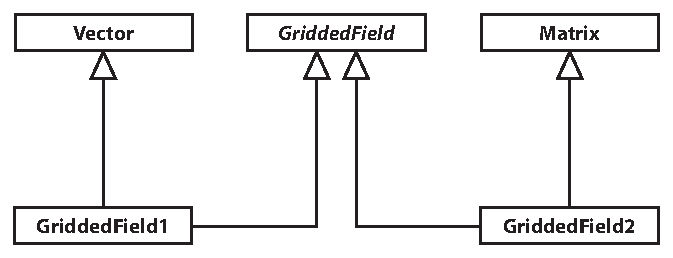
\includegraphics{Figs/development/griddedfields_inheritance}
\caption{UML diagram of gridded field inheritance.}
\zlabel{fig:griddedfields:uml}
\end{center}
\end{figure}


\section{Constructing Gridded Fields}
%-------------------------------------------------------------------------
\zlabel{sec:griddedfields:construct}


\subsection{Creation}
%-------------------------------------------------------------------------
\zlabel{sec:griddedfields:create}

Each \artsstyle{GriddedFieldX} offers two constructors. One default constructor that creates an unnamed gridded field and a second constructor that takes a String with the name of the gridded field as an argument.

\begin{verbatim}
  GriddedField1 gfone("I'm a GriddedField1");
  GriddedField2 gftwo;
  
  gftwo.set_name ("I'm a GriddedField2");
\end{verbatim}


\subsection{Initializing the grids}
%-------------------------------------------------------------------------
\zlabel{sec:griddedfields:initgrids}

Once a gridded field has been created, we can start setting up the grids. There are two different types of grids, a numeric grid and a string grid.

\begin{verbatim}
Vector gfonegrid(1,5,1);        // gfonegrid = [1,2,3,4,5]
gfone.set_grid(0, gfonegrid);   // Set grid for the vector elements

MakeArray<String> gftwogrid0("Channel 1", "Channel2", "Channel3");
Vector gftwogrid1(1,5,1);       // gftwogrid1 = [1,2,3,4,5]

gftwo.set_grid(0, gftwogrid0);  // Set grid for the matrix rows
gftwo.set_grid(1, gftwogrid1);  // Set grid for the matrix columns
\end{verbatim}

Note that the first grid corresponds to the highest dimension of the data. This means grid 0 in a \artsstyle{GriddedField2} corresponds to the rows of the matrix. Grid 1 corresponds to the columns.

In addition to the grid values, a name can be assigned to each grid.

\begin{verbatim}
gfone.set_grid_name (0, "Pressure");

gftwo.set_grid_name (0, "Instrument channel");
gftwo.set_grid_name (1, "Pressure");
\end{verbatim}

\subsection{Initializing the data}
%-------------------------------------------------------------------------
\zlabel{sec:griddedfields:initdata}

Because gridded fields do not only inherit from \artsstyle{GriddedField} but also from the class of the data they contain, it is possible to treat them in exactly the same way. See Figure \zref{fig:griddedfields:objects}.

\begin{figure}[ht!]
\begin{center}
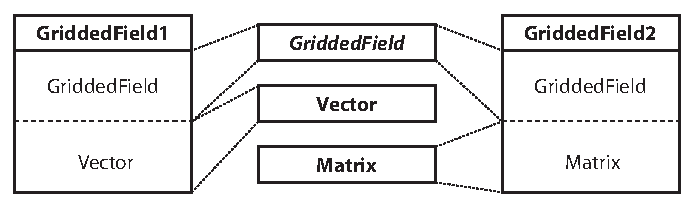
\includegraphics{Figs/development/griddedfields_objects}
\caption{Visualization of gridded field objects.}
\zlabel{fig:griddedfields:objects}
\end{center}
\end{figure}

Let us take the \artsstyle{gfone} variable from the previous examples. \artsstyle{gfone} is a \artsstyle{GriddedField1} which means it has \artsstyle{GriddedField} and \artsstyle{Vector} as superclasses. Polymorphism allows us to use a \artsstyle{GriddedField1} in every place where it is valid to use a \artsstyle{Vector}. The only requirement is to cast the gridded field to the corresponding data type.

\begin{verbatim}
Vector avector(1,5,0.5);    // avector = [1,1.5,2,2.5,3]

(Vector&)gfone = avector;

Matrix amatrix(2,3,4.);     // amatrix = [[4,4,4],[4,4,4]]

(Matrix&)gftwo = amatrix;
\end{verbatim}

\subsection{Consistency check}
%-------------------------------------------------------------------------
\zlabel{sec:griddedfields:consistency}

After initializing or changing either the grids or the data, it can happen that the size of the grids does not match up with the size of the data anymore. Each gridded field provides a convenience function which can be called to make a consistency check.

\begin{verbatim}
if (!gfone.checksize())
  cout << gfone.get_name()
       << ": Sizes of grid and data don't match" << endl;

// This should fail!
if (!gftwo.checksize())
  cout << gftwo.get_name()
       << ": Sizes of grids and data don't match" << endl;
\end{verbatim}

%%% Local Variables:
%%% mode: latex
%%% TeX-master: "arts_developer"
%%% End:

